\fontsize{9}{10.5}\selectfont

\par\Needspace{120pt}\medskip
\section*{Paper 5: AY2024/\allowbreak{}25 Semester 1 --- Collaborative task management}\label{paper-2425-s1}
\phantomsection\addcontentsline{toc}{section}{Paper 5: AY2024/25 Semester 1 --- Collaborative task management}\markboth{AY2024/25 S1}{}
\sectionlabel{h-181-ay202425-semester-1--collaborative-task-management}
\textbf{Source:} \href{run:/Users/bryangoh/Work/ntu-cs/sc2006/pyps/SC2006\_AY2425\_S1\_Questions.pdf}{Question paper}, Q1--Q4 on PDF pp. 1--3; Appendix A on p. 4.




\begin{studycolumns}
\vspace{0pt}
\textbf{Case facts.} Registered users log in; access is role based. Members create tasks; team leaders/\allowbreak{}project managers verify and assign them to an individual or team, setting deadlines/\allowbreak{}milestones. Tasks have categories, priorities and tags. Reassignment is allowed, but a task cannot have two assignments simultaneously. Finished tasks can be updated/\allowbreak{}deleted. Chat, comments and documents support collaboration; dashboards show progress/\allowbreak{}overdue work/\allowbreak{}workloads; email and in-app notifications cover deadlines, upcoming tasks and priority changes, with configurable alerts.

\needspace{4\baselineskip}
\subsection*{Q1 --- Use cases (25 marks)}
\sectionlabel{h-q1--use-cases-25-marks-4}
\textbf{(a) Actors/\allowbreak{}use cases/\allowbreak{}relationships (19). (b) Task-assignment use case with actors, preconditions and alternative flows (6).}


\textbf{(a)} Actors: Team Member, Team Leader, Project Manager and external Email Server. Leaders/\allowbreak{}managers have member capabilities; model actor generalization in UML. The dashboard and notification subsystem are internal, not actors.
\end{studycolumns}


\par\smallskip\noindent\begin{minipage}{\linewidth}\centering
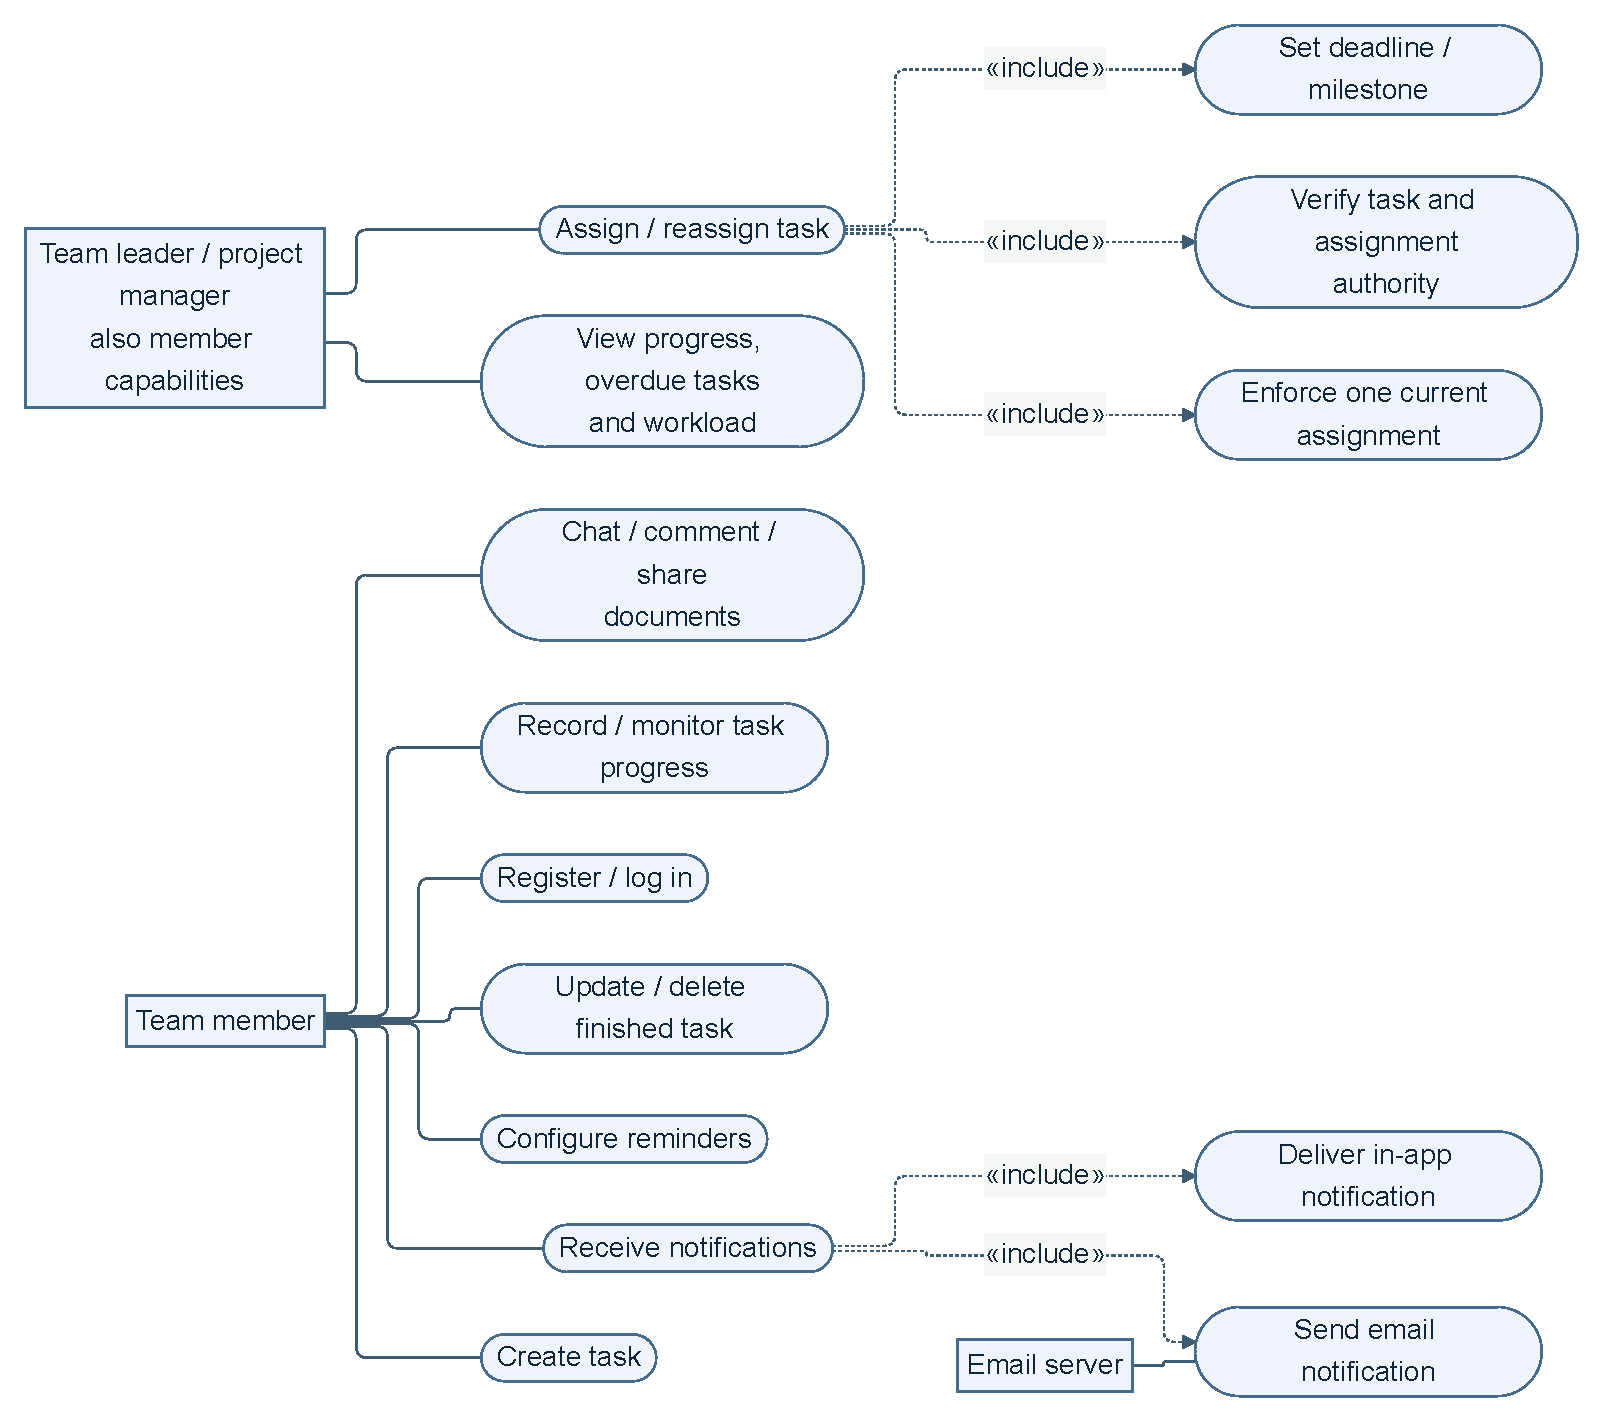
\includegraphics[width=451.44pt]{images/fig-069.pdf}
\captionof{figure}{Q1 --- Use cases (25 marks)}\end{minipage}\par\smallskip

\begin{studycolumns}
\vspace{0pt}



Every protected action requires a valid session and appropriate role. Member permissions for modifying/\allowbreak{}deleting tasks must follow the agreed access policy; the appendix does not say every member can modify every task. Include categorisation/\allowbreak{}priority/\allowbreak{}tag fields in Create/\allowbreak{}Update Task descriptions rather than treating each field entry as a separate user goal. No optional extension is needed simply to satisfy the diagram wording.

\textbf{(b) Use case: Assign Task.} Primary actor: authenticated Team Leader or Project Manager. Preconditions: task exists and actor is authorised; chosen individual/\allowbreak{}team exists. Normal flow: actor selects task; system presents task and current assignment; actor verifies task, chooses one assignee and specifies deadline/\allowbreak{}milestones; system validates rights and details; system atomically records the assignment and exposes updated workload/\allowbreak{}progress. Alternatives: unverified/\allowbreak{}invalid task or unavailable assignee, request correction; unauthorised actor, reject; concurrent assignment change, reject/\allowbreak{}reload; reassignment, replace the old assignment atomically instead of appending a second active assignment. \textbf{Assumption:} ``one assignment'' means one assignee target, which may be an individual or a team, not only one person within a team.

\needspace{4\baselineskip}
\subsection*{Q2 --- Analysis, lifecycle and process (25 marks)}
\sectionlabel{h-q2--analysis-lifecycle-and-process-25-marks}
\textbf{(a) Assignment conceptual classes/\allowbreak{}stereotypes (9). (b) Activity/\allowbreak{}swimlane diagram from task creation to deletion (7). (c) Waterfall response to drastic mid-project requirement change (4). (d) Improve customer satisfaction after a disappointing first agile sprint (5).}


\textbf{(a)}
\end{studycolumns}


\par\smallskip\noindent\begin{minipage}{\linewidth}\centering
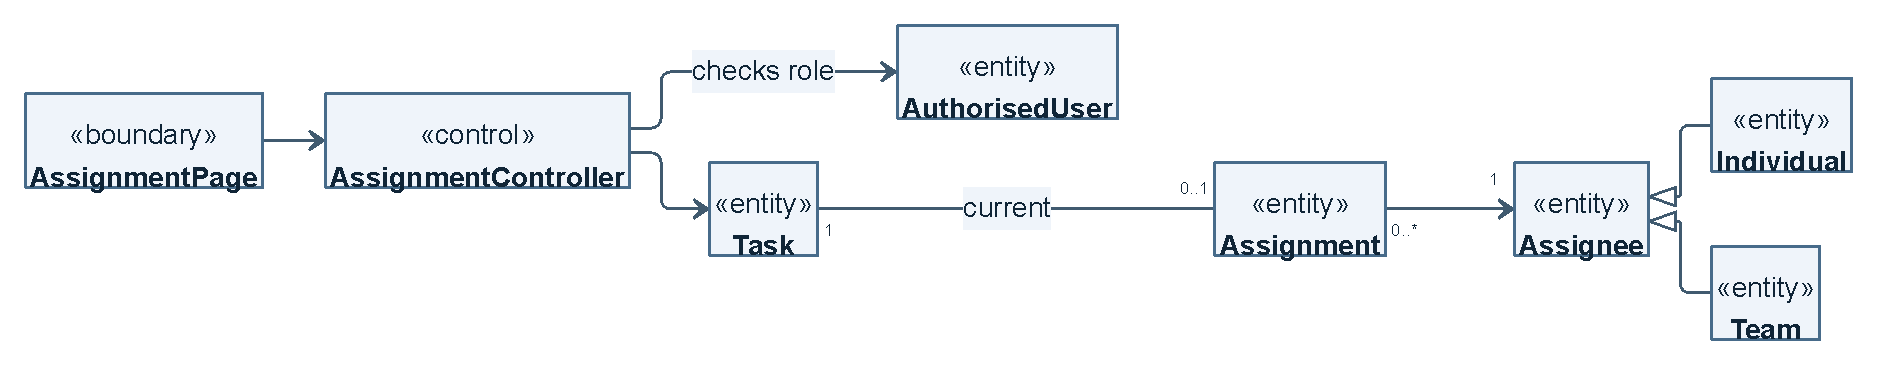
\includegraphics[width=514.00pt]{images/fig-070.pdf}
\captionof{figure}{Q2 --- Analysis, lifecycle and process (25 marks)}\end{minipage}\par\smallskip



If assignment history is added, use \code{0.\allowbreak{}.\allowbreak{}*} historical assignments plus an explicit \textbf{at most one active assignment} constraint; do not remove the invariant.

\textbf{(b)} The appendix permits update/\allowbreak{}deletion after completion, so those actions appear after Finished. Reassignment is an atomic replacement. Deletion is optional, not an automatic consequence of finishing.







\par\smallskip\noindent\begin{minipage}{\linewidth}\centering
{\scriptsize\textbf{A: create, verify and assign}}\par\smallskip
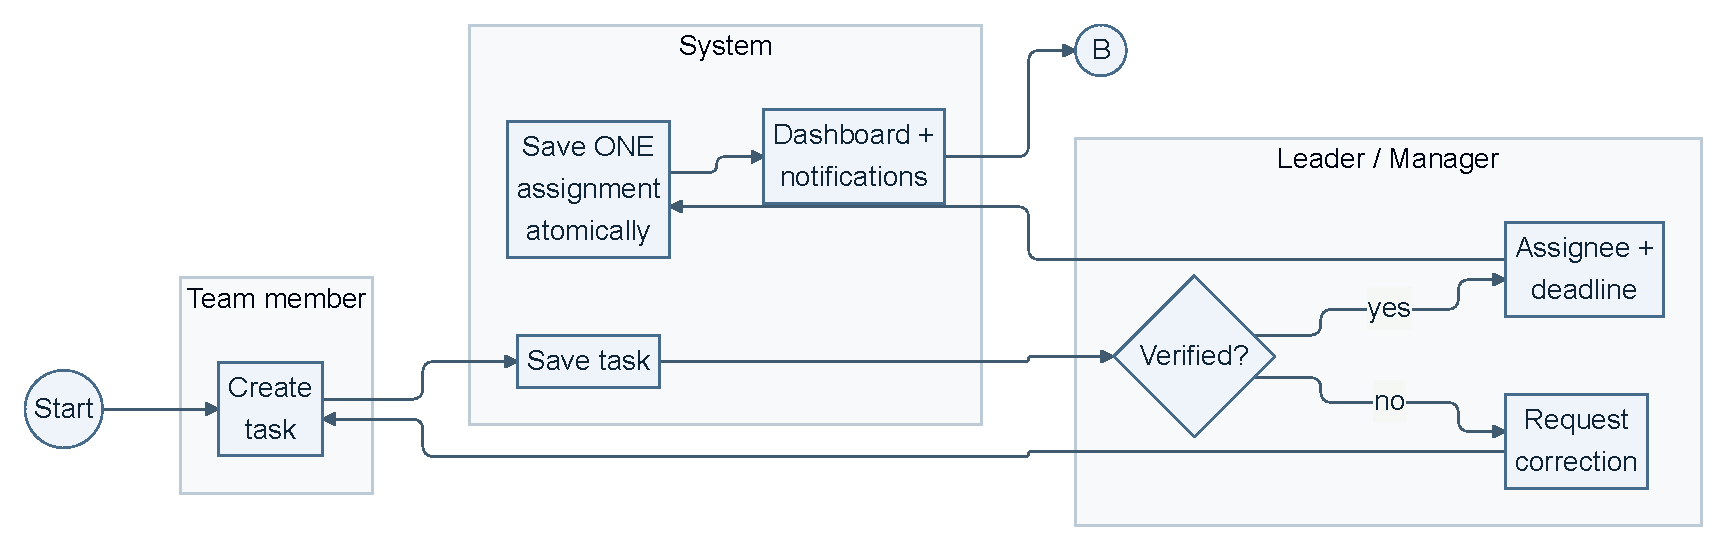
\includegraphics[width=442.00pt]{images/fig-071-a.pdf}\par\smallskip
{\scriptsize\textbf{B: work, reassign or finish}}\par\smallskip
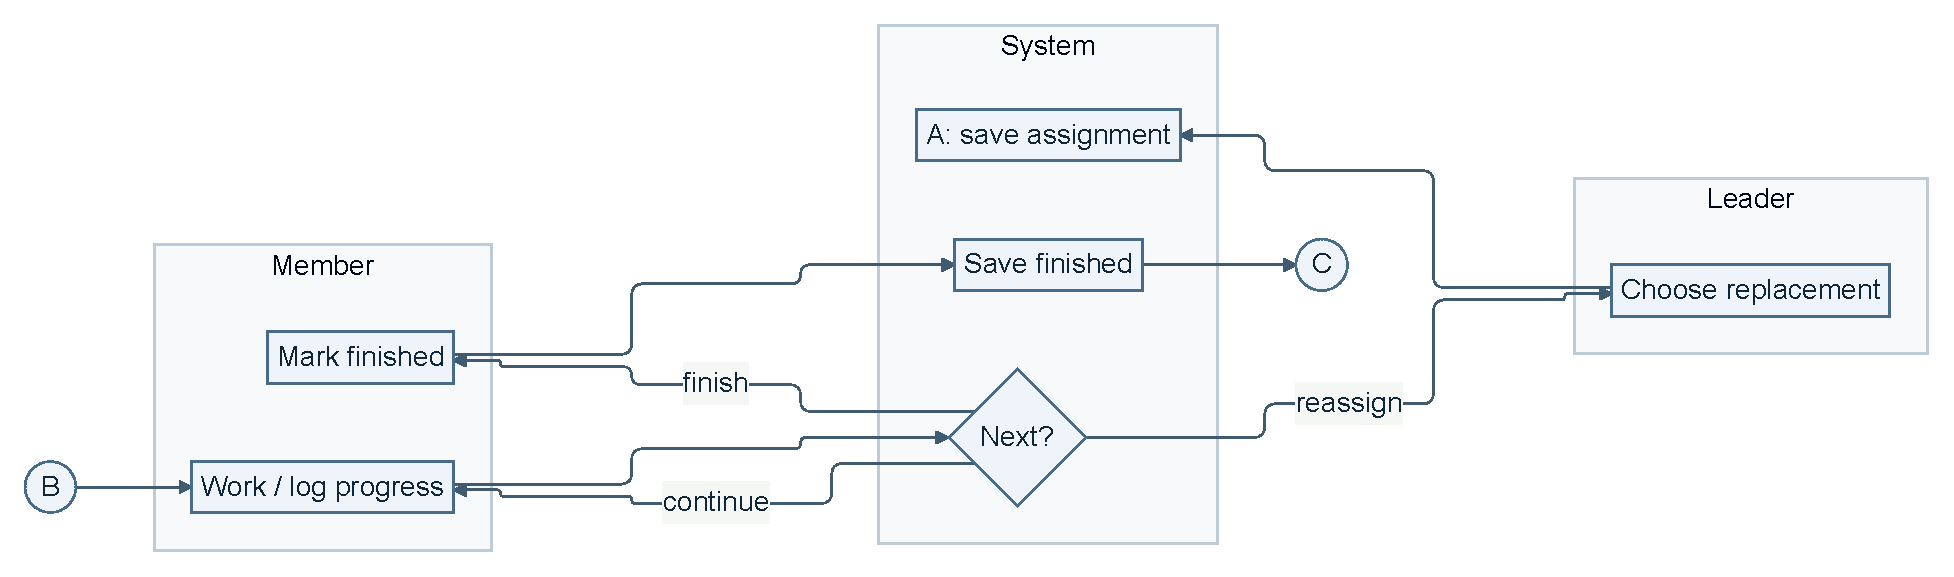
\includegraphics[width=500.00pt]{images/fig-071-b.pdf}\par\smallskip
{\scriptsize\textbf{C: authorised finished-task actions}}\par\smallskip
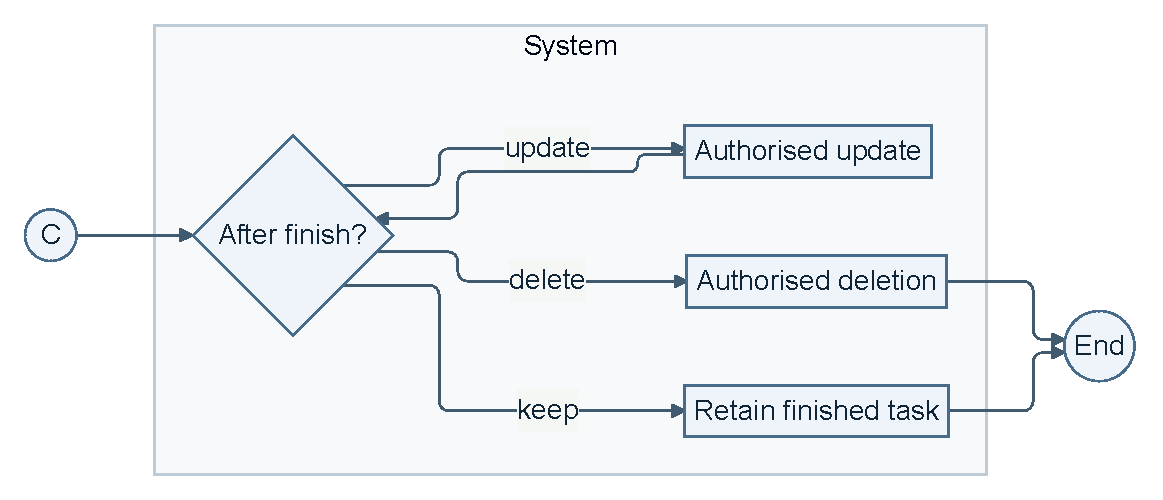
\includegraphics[width=297.20pt]{images/fig-071-c.pdf}\par\smallskip
\captionof{figure}{Q2 --- Analysis, lifecycle and process (25 marks) --- B/C continue below; A returns to atomic assignment.}\end{minipage}\par\smallskip

\begin{studycolumns}
\vspace{0pt}













\textbf{(c)} Apply \hyperref[answer-waterfall]{W, p.\ \pageref{answer-waterfall}} to the drastic task-system change; update affected artefacts and agree revised scope/schedule. Persistent change may justify incremental/agile delivery.

\textbf{(d)} Apply \hyperref[answer-scrum]{S, p.\ \pageref{answer-scrum}}: clarify unmet needs/acceptance criteria, reprioritise value with the PO, choose smaller usable increments and retrospect on estimates/capacity/integration.

\needspace{4\baselineskip}
\subsection*{Q3 --- Architecture, NFR and patterns (25 marks)}
\sectionlabel{h-q3--architecture-nfr-and-patterns-25-marks}
\textbf{(a)(i) Detailed architecture/\allowbreak{}classes (8); (ii) one relevant NFR and alternative architecture addressing it (8). (b)(i) Combined-pattern scenario/\allowbreak{}classes (6); (ii) is combining patterns always beneficial? (3).}


\textbf{(a)(i)} Use a layered task application: UI boundaries, application services, task/\allowbreak{}assignment entities and repositories/\allowbreak{}notification gateways.
\end{studycolumns}


\par\smallskip\noindent\begin{minipage}{\linewidth}\centering
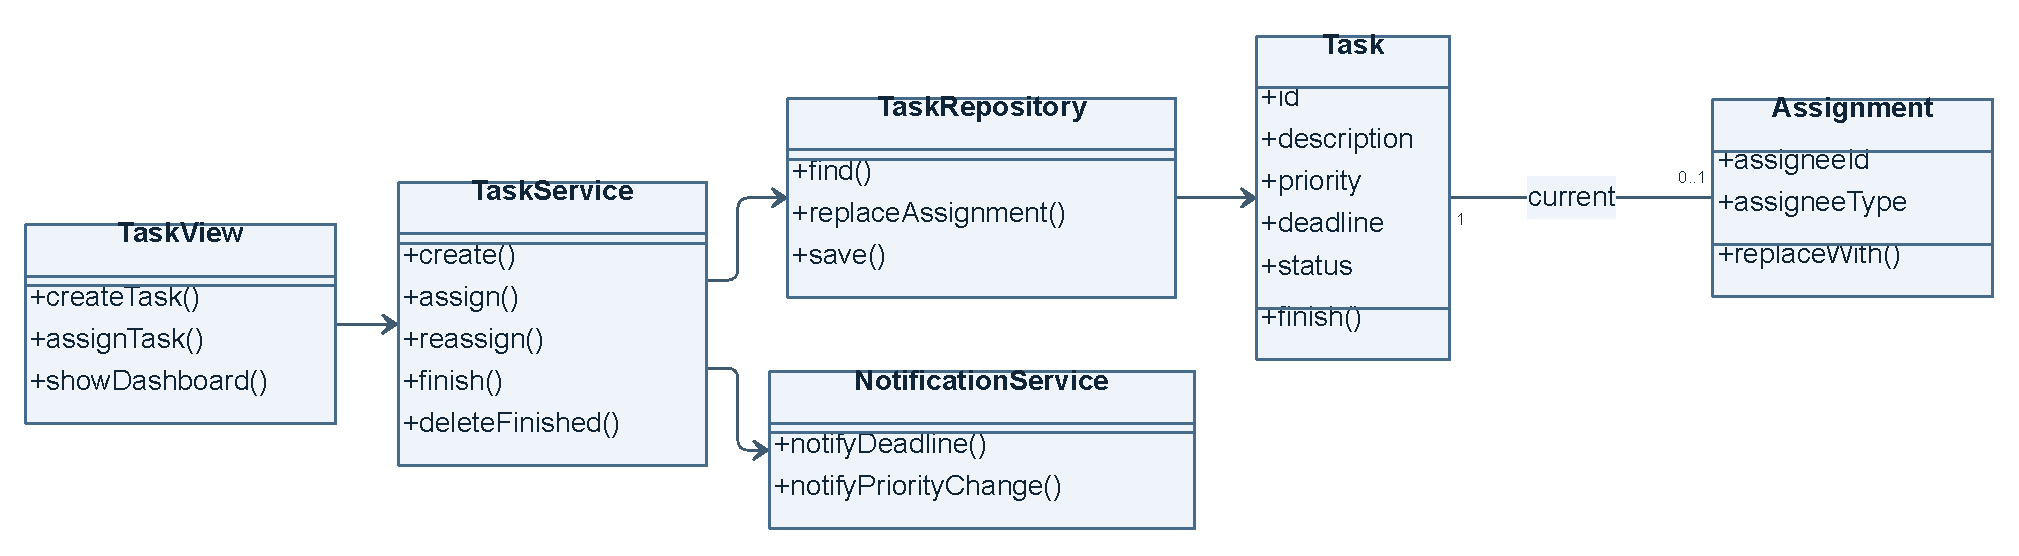
\includegraphics[width=514.00pt]{images/fig-072.pdf}
\captionof{figure}{Q3 --- Architecture, NFR and patterns (25 marks) --- assignment replacement is atomic}\end{minipage}\par\smallskip



\textbf{(a)(ii)} Choose \textbf{security/\allowbreak{}access control}, explicitly motivated by role-based access and sensitive team information. An alternative centralised \textbf{client--server architecture with a security Facade} places all task operations behind authenticated server-side authorisation. Browser/\allowbreak{}UI role checks alone cannot protect the data.




\par\smallskip\noindent\begin{minipage}{\linewidth}\centering
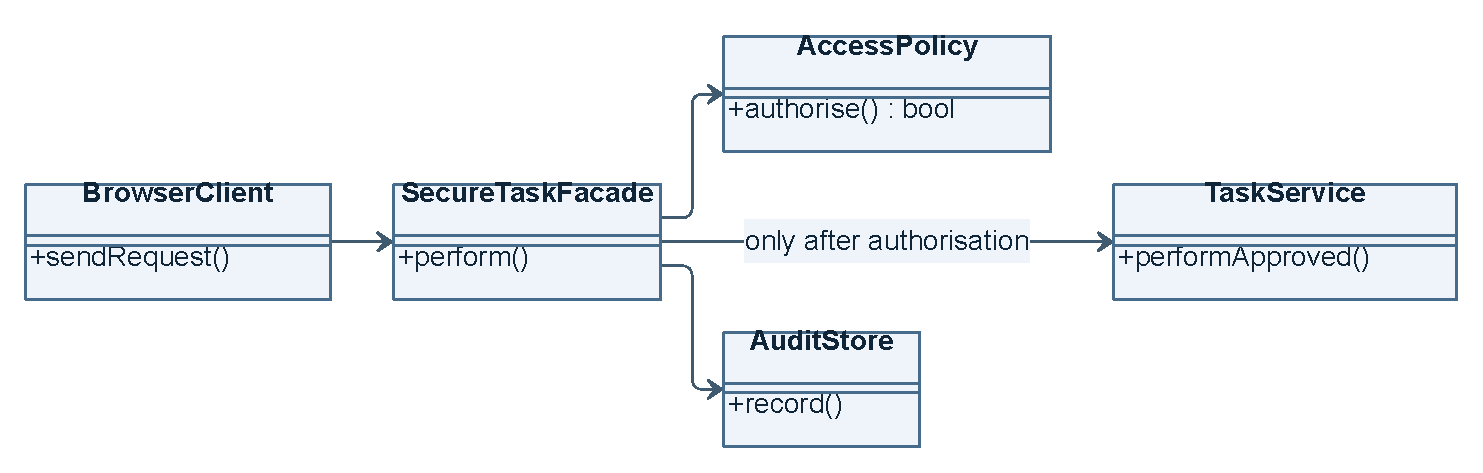
\includegraphics[width=417.56pt]{images/fig-073.pdf}
\captionof{figure}{Q3 --- Architecture, NFR and patterns (25 marks)}\end{minipage}\par\smallskip

\begin{studycolumns}
\vspace{0pt}



Keep Task/\allowbreak{}Assignment/\allowbreak{}Repository from Q3(a)(i) behind TaskService. Centralisation makes policy consistent across clients and supports audited denials; it adds a server/\allowbreak{}network dependency. Audit storage is a proposed security measure, not an explicit appendix feature. Layering and client--server are compatible architectural dimensions; the alternative adds a trust boundary rather than claiming that these styles are mutually exclusive.

\textbf{(b)(i)} Combine Observer with Simple Factory for email and in-app notifications. A task subject notifies both subscribed channels on relevant events; a factory creates/\allowbreak{}configures channel observers. Deadline timers also publish events rather than requiring a task to mutate every second.
\end{studycolumns}


\par\smallskip\noindent\begin{minipage}{\linewidth}\centering
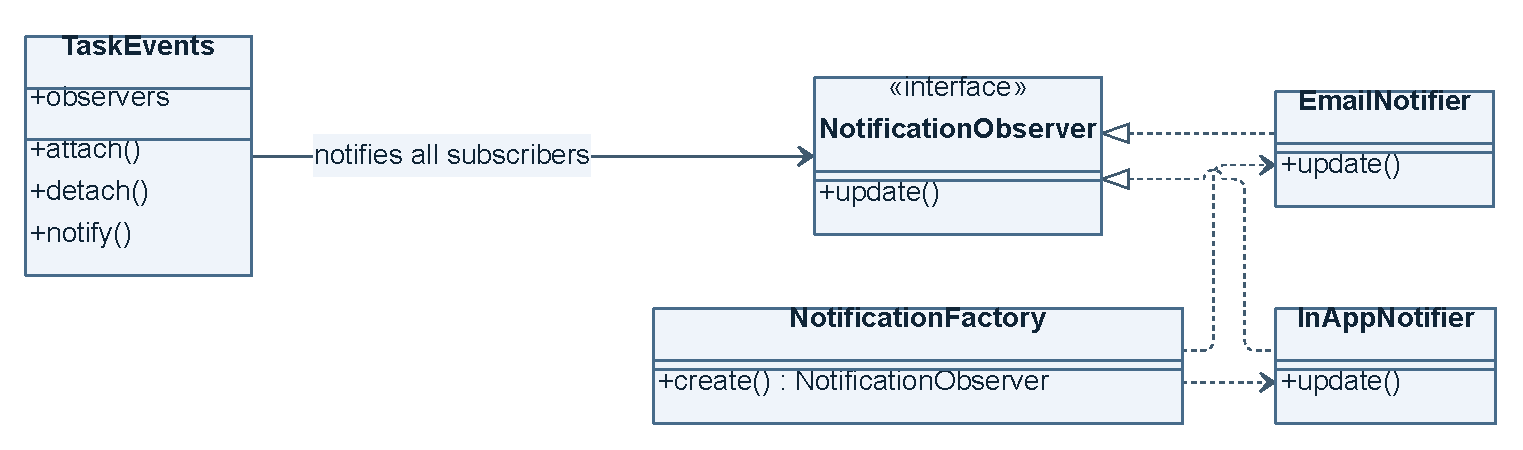
\includegraphics[width=428.56pt]{images/fig-074.pdf}
\captionof{figure}{Q3 --- Architecture, NFR and patterns (25 marks)}\end{minipage}\par\smallskip

\begin{studycolumns}
\vspace{0pt}



Factory governs creation; Observer governs runtime notification without coupling task code to concrete delivery channels. The requirements call for email \textbf{and} in-app messages, not arbitrarily selecting only one.

\textbf{(b)(ii)} No: apply \hyperref[answer-pattern-cost]{C, p.\ \pageref{answer-pattern-cost}}. Email and in-app notifications justify separate channels; unrelated patterns add cost without solving another force.

\needspace{4\baselineskip}
\subsection*{Q4 --- Task inputs, shift-left and maintenance (25 marks)}
\sectionlabel{h-q4--task-inputs-shift-left-and-maintenance-25-marks}
\textbf{(a)(i) Derive ECs for Task Description, Resource needed, Deadline and Task Priority (4). (ii) Give on/\allowbreak{}below/\allowbreak{}above boundary values (4). (iii) Design defensive tests (5).}


\textbf{Input interpretation.} Task Description must be ASCII; Resource needed is a 4-digit integer; Deadline is between 2024 and 2026; Task Priority is one of \code{Critical}, \code{High}, \code{Normal}, \code{Low}, \code{Very Low}. Assume a positive 4-digit numeric value (not a string whose leading zeroes count as digits), inclusive complete calendar years, and one-day date resolution. These interpretations are stated because the brief does not specify parsing details. Do not invent an ASCII-field length limit.

\textbf{(i) Equivalence classes:}
\end{studycolumns}


{\fontsize{8.5}{9.8}\selectfont
\begin{longtable}{L{\dimexpr 0.22368\linewidth-5.37pt\relax}L{\dimexpr 0.33177\linewidth-7.96pt\relax}L{\dimexpr 0.44455\linewidth-10.67pt\relax}}
\toprule
\rowcolor{ice}\textbf{Field} & \textbf{Valid EC} & \textbf{Invalid ECs} \\
\midrule\endfirsthead
\toprule\rowcolor{ice}\textbf{Field} & \textbf{Valid EC} & \textbf{Invalid ECs} \\
\midrule\endhead
\multicolumn{3}{r}{\scriptsize Continued on next page}\\\endfoot
\bottomrule\endlastfoot
Task Description & ASCII text & Text containing non-ASCII characters \\
Resource needed & Integer 1000\ldots{}9999 & Integer below 1000; integer above 9999; malformed/\allowbreak{}non-integer input at the input boundary \\
Deadline & Real calendar date 2024-01-01\ldots{}2026-12-31 & Real date before 2024-01-01; real date after 2026-12-31; malformed/\allowbreak{}nonexistent date \\
Task Priority & One EC containing \{Critical, High, Normal, Low, Very Low\} & Any unlisted value \\
\end{longtable}
}

The category set is \textbf{one valid EC}, although testing all its few members is useful. No empty-string prohibition or printable-only ASCII restriction is supplied; clarify those separately instead of asserting an invented oracle.

\textbf{(ii) Boundary triplets:}




{\fontsize{8.5}{9.8}\selectfont
\begin{longtable}{L{\dimexpr 0.27680\linewidth-8.86pt\relax}L{\dimexpr 0.23890\linewidth-7.64pt\relax}L{\dimexpr 0.24215\linewidth-7.75pt\relax}L{\dimexpr 0.24215\linewidth-7.75pt\relax}}
\toprule
\rowcolor{ice}\textbf{Field /\allowbreak{} boundary} & \textbf{Just below} & \textbf{On boundary} & \textbf{Just above} \\
\midrule\endfirsthead
\toprule\rowcolor{ice}\textbf{Field /\allowbreak{} boundary} & \textbf{Just below} & \textbf{On boundary} & \textbf{Just above} \\
\midrule\endhead
\multicolumn{4}{r}{\scriptsize Continued on next page}\\\endfoot
\bottomrule\endlastfoot
Resource needed: minimum & 999 (reject) & 1000 (accept) & 1001 (accept) \\
Resource needed: maximum & 9998 (accept) & 9999 (accept) & 10000 (reject) \\
Deadline: earliest & 2023-12-31 (reject) & 2024-01-01 (accept) & 2024-01-02 (accept) \\
Deadline: latest & 2026-12-30 (accept) & 2026-12-31 (accept) & 2027-01-01 (reject) \\
\end{longtable}
}

ASCII membership and unordered categories have no specified application-level ordered boundary. Malformed values are additional EC tests, not numeric/\allowbreak{}date neighbours.

\textbf{(iii) Defensive suite.} Use the common testing conventions below; valid rows combine boundaries, invalid rows isolate one field. The full boundary suite is retained.




{\fontsize{8.5}{9.8}\selectfont
\begin{longtable}{L{\dimexpr 0.18631\linewidth-7.45pt\relax}L{\dimexpr 0.16907\linewidth-6.76pt\relax}L{\dimexpr 0.16907\linewidth-6.76pt\relax}L{\dimexpr 0.16907\linewidth-6.76pt\relax}L{\dimexpr 0.30647\linewidth-12.26pt\relax}}
\toprule
\rowcolor{ice}\textbf{Task Description} & \textbf{Resource needed} & \textbf{Deadline} & \textbf{Task Priority} & \textbf{Expected /\allowbreak{} purpose} \\
\midrule\endfirsthead
\toprule\rowcolor{ice}\textbf{Task Description} & \textbf{Resource needed} & \textbf{Deadline} & \textbf{Task Priority} & \textbf{Expected /\allowbreak{} purpose} \\
\midrule\endhead
\multicolumn{5}{r}{\scriptsize Continued on next page}\\\endfoot
\bottomrule\endlastfoot
\code{Implement API} & \code{1000} & \code{2024-\allowbreak{}01-\allowbreak{}01} & \code{Critical} & Accept --- valid boundaries /\allowbreak{} category coverage \\
\code{Implement API} & \code{1001} & \code{2024-\allowbreak{}01-\allowbreak{}02} & \code{High} & Accept --- valid boundaries /\allowbreak{} category coverage \\
\code{Implement API} & \code{9998} & \code{2026-\allowbreak{}12-\allowbreak{}30} & \code{Normal} & Accept --- valid boundaries /\allowbreak{} category coverage \\
\code{Implement API} & \code{9999} & \code{2026-\allowbreak{}12-\allowbreak{}31} & \code{Low} & Accept --- valid boundaries /\allowbreak{} category coverage \\
\code{Implement API} & \code{5499} & \code{2025-\allowbreak{}07-\allowbreak{}01} & \code{Very Low} & Accept --- interior baseline /\allowbreak{} category coverage \\
\code{caf\'{e}} & \code{5499} & \code{2025-\allowbreak{}07-\allowbreak{}01} & \code{Critical} & Reject --- non-ASCII Task Description \\
\code{Implement API} & \code{999} & \code{2025-\allowbreak{}07-\allowbreak{}01} & \code{Critical} & Reject --- Resource needed below minimum \\
\code{Implement API} & \code{10000} & \code{2025-\allowbreak{}07-\allowbreak{}01} & \code{Critical} & Reject --- Resource needed above maximum \\
\code{Implement API} & \code{5499} & \code{2023-\allowbreak{}12-\allowbreak{}31} & \code{Critical} & Reject --- Deadline below minimum \\
\code{Implement API} & \code{5499} & \code{2027-\allowbreak{}01-\allowbreak{}01} & \code{Critical} & Reject --- Deadline above maximum \\
\code{Implement API} & \code{5499} & \code{2025-\allowbreak{}07-\allowbreak{}01} & \code{Unknown} & Reject --- unlisted Task Priority \\
\code{Implement API} & \code{12x} & \code{2025-\allowbreak{}07-\allowbreak{}01} & \code{Critical} & Reject --- malformed integer; extra defensive case \\
\code{Implement API} & \code{5499} & \code{2024-\allowbreak{}02-\allowbreak{}30} & \code{Critical} & Reject --- nonexistent calendar date; extra defensive case \\
\end{longtable}
}

\begin{studycolumns}
\vspace{0pt}

\textbf{(b) Why is shift-left testing useful? (4). (c) Four maintenance challenges and mitigations (8).}


\textbf{(b)} Reviewing requirements and designing tests early exposes ambiguity before it spreads into design/\allowbreak{}code. Early unit/\allowbreak{}integration automation provides fast feedback, reduces downstream rework and makes changes safer. Examples: identify the one-assignment invariant during analysis and test the service before building the dashboard. Shift-left complements rather than eliminates later system, performance and acceptance testing.

\textbf{(c)}
\end{studycolumns}


{\fontsize{8.5}{9.8}\selectfont
\begin{longtable}{L{\dimexpr 0.38681\linewidth-6.19pt\relax}L{\dimexpr 0.61319\linewidth-9.81pt\relax}}
\toprule
\rowcolor{ice}\textbf{Challenge} & \textbf{Mitigation} \\
\midrule\endfirsthead
\toprule\rowcolor{ice}\textbf{Challenge} & \textbf{Mitigation} \\
\midrule\endhead
\multicolumn{2}{r}{\scriptsize Continued on next page}\\\endfoot
\bottomrule\endlastfoot
Understanding unfamiliar/\allowbreak{}poorly documented legacy code & Maintain architecture/\allowbreak{}decision notes, clear interfaces and traceable change history; use code reviews and onboarding. \\
Regressions caused by changes & Automate regression tests, check integration/\allowbreak{}compatibility, and use reviewed version-controlled changes with rollback. \\
Increasing technical debt and coupling & Refactor incrementally with behaviour-preservation checks; keep responsibilities and boundaries clear. \\
Changing requirements/\allowbreak{}dependencies and operational environments & Perform impact analysis, prioritise changes, maintain supported dependency versions, and update requirements/\allowbreak{}tests/\allowbreak{}documentation together. \\
\end{longtable}
}

Tie each challenge to its remedy rather than listing four generic ``best practices'' without explanation.


\par\Needspace{120pt}\medskip
\section*{Paper 6: AY2024/\allowbreak{}25 Semester 2 --- Disaster Warning System (DWS)}\label{paper-2425-s2}
\phantomsection\addcontentsline{toc}{section}{Paper 6: AY2024/25 Semester 2 --- Disaster Warning System (DWS)}\markboth{AY2024/25 S2}{}
\sectionlabel{h-182-ay202425-semester-2--disaster-warning-system-dws}
\textbf{Source:} \href{run:/Users/bryangoh/Work/ntu-cs/sc2006/pyps/SC2006\_AY2425\_S2\_Questions.pdf}{Question paper}, Q1--Q4 on PDF pp. 1--4; Appendix A on p. 5.




\begin{studycolumns}
\vspace{0pt}
\textbf{Case facts.} A local government deploys a configurable DWS. Its manager registers/\allowbreak{}deregisters physically connected sensors and alert systems, links/\allowbreak{}unlinks registered sensor--alert pairs, and chooses safe measurement ranges. Registered sensors send integer updates at any time; an out-of-range value triggers the linked alert. Changes and received/\allowbreak{}sent messages are recorded. More than 24 hours without an update from a registered sensor causes a manager alert. The manager can retrieve the full record.

\needspace{4\baselineskip}
\subsection*{Q1 --- Stakeholders, requirements and use cases (25 marks)}
\sectionlabel{h-q1--stakeholders-requirements-and-use-cases-25-marks}
\textbf{(a) Four stakeholders and interests (4). (b) Three FRs and three NFRs (6). (c) Actors/\allowbreak{}use cases/\allowbreak{}relationships (15).}


\textbf{(a)} Local government: public safety, budget and dependable operation. DWS manager: correct configuration, sensor health and usable records. Emergency responders/\allowbreak{}alert recipients: timely, accurate, actionable warnings. Residents: protection from disasters and avoidance of missed/\allowbreak{}false alarms. A stakeholder need not directly operate the software and therefore need not be an actor.

\textbf{(b) Three FRs:} (1) accept sensor/\allowbreak{}alert registration only when physical connection is detected; (2) maintain configured links/\allowbreak{}ranges and trigger linked alerts for out-of-range integer measurements; (3) notify the manager when a registered sensor has supplied no update for over 24 hours. Recording and record retrieval are additional FRs.

\textbf{Three proposed NFRs:} (1) flexibility/\allowbreak{}interoperability across different deployments and sensor/\allowbreak{}alert implementations; (2) availability/\allowbreak{}reliability for ongoing monitoring and fault recovery; (3) performance for timely processing and delivery of alerts under the agreed peak sensor workload. Flexibility is explicit in the case; measurable availability, latency and recovery targets must be agreed, not invented. ``Log all messages'' is functional behaviour, not automatically an NFR merely because it concerns auditing.

\textbf{(c)} Actors: DWS Manager, external Sensor, external Alert System. Time passage is an event, not necessarily an actor.
\end{studycolumns}


\par\smallskip\noindent\begin{minipage}{\linewidth}\centering
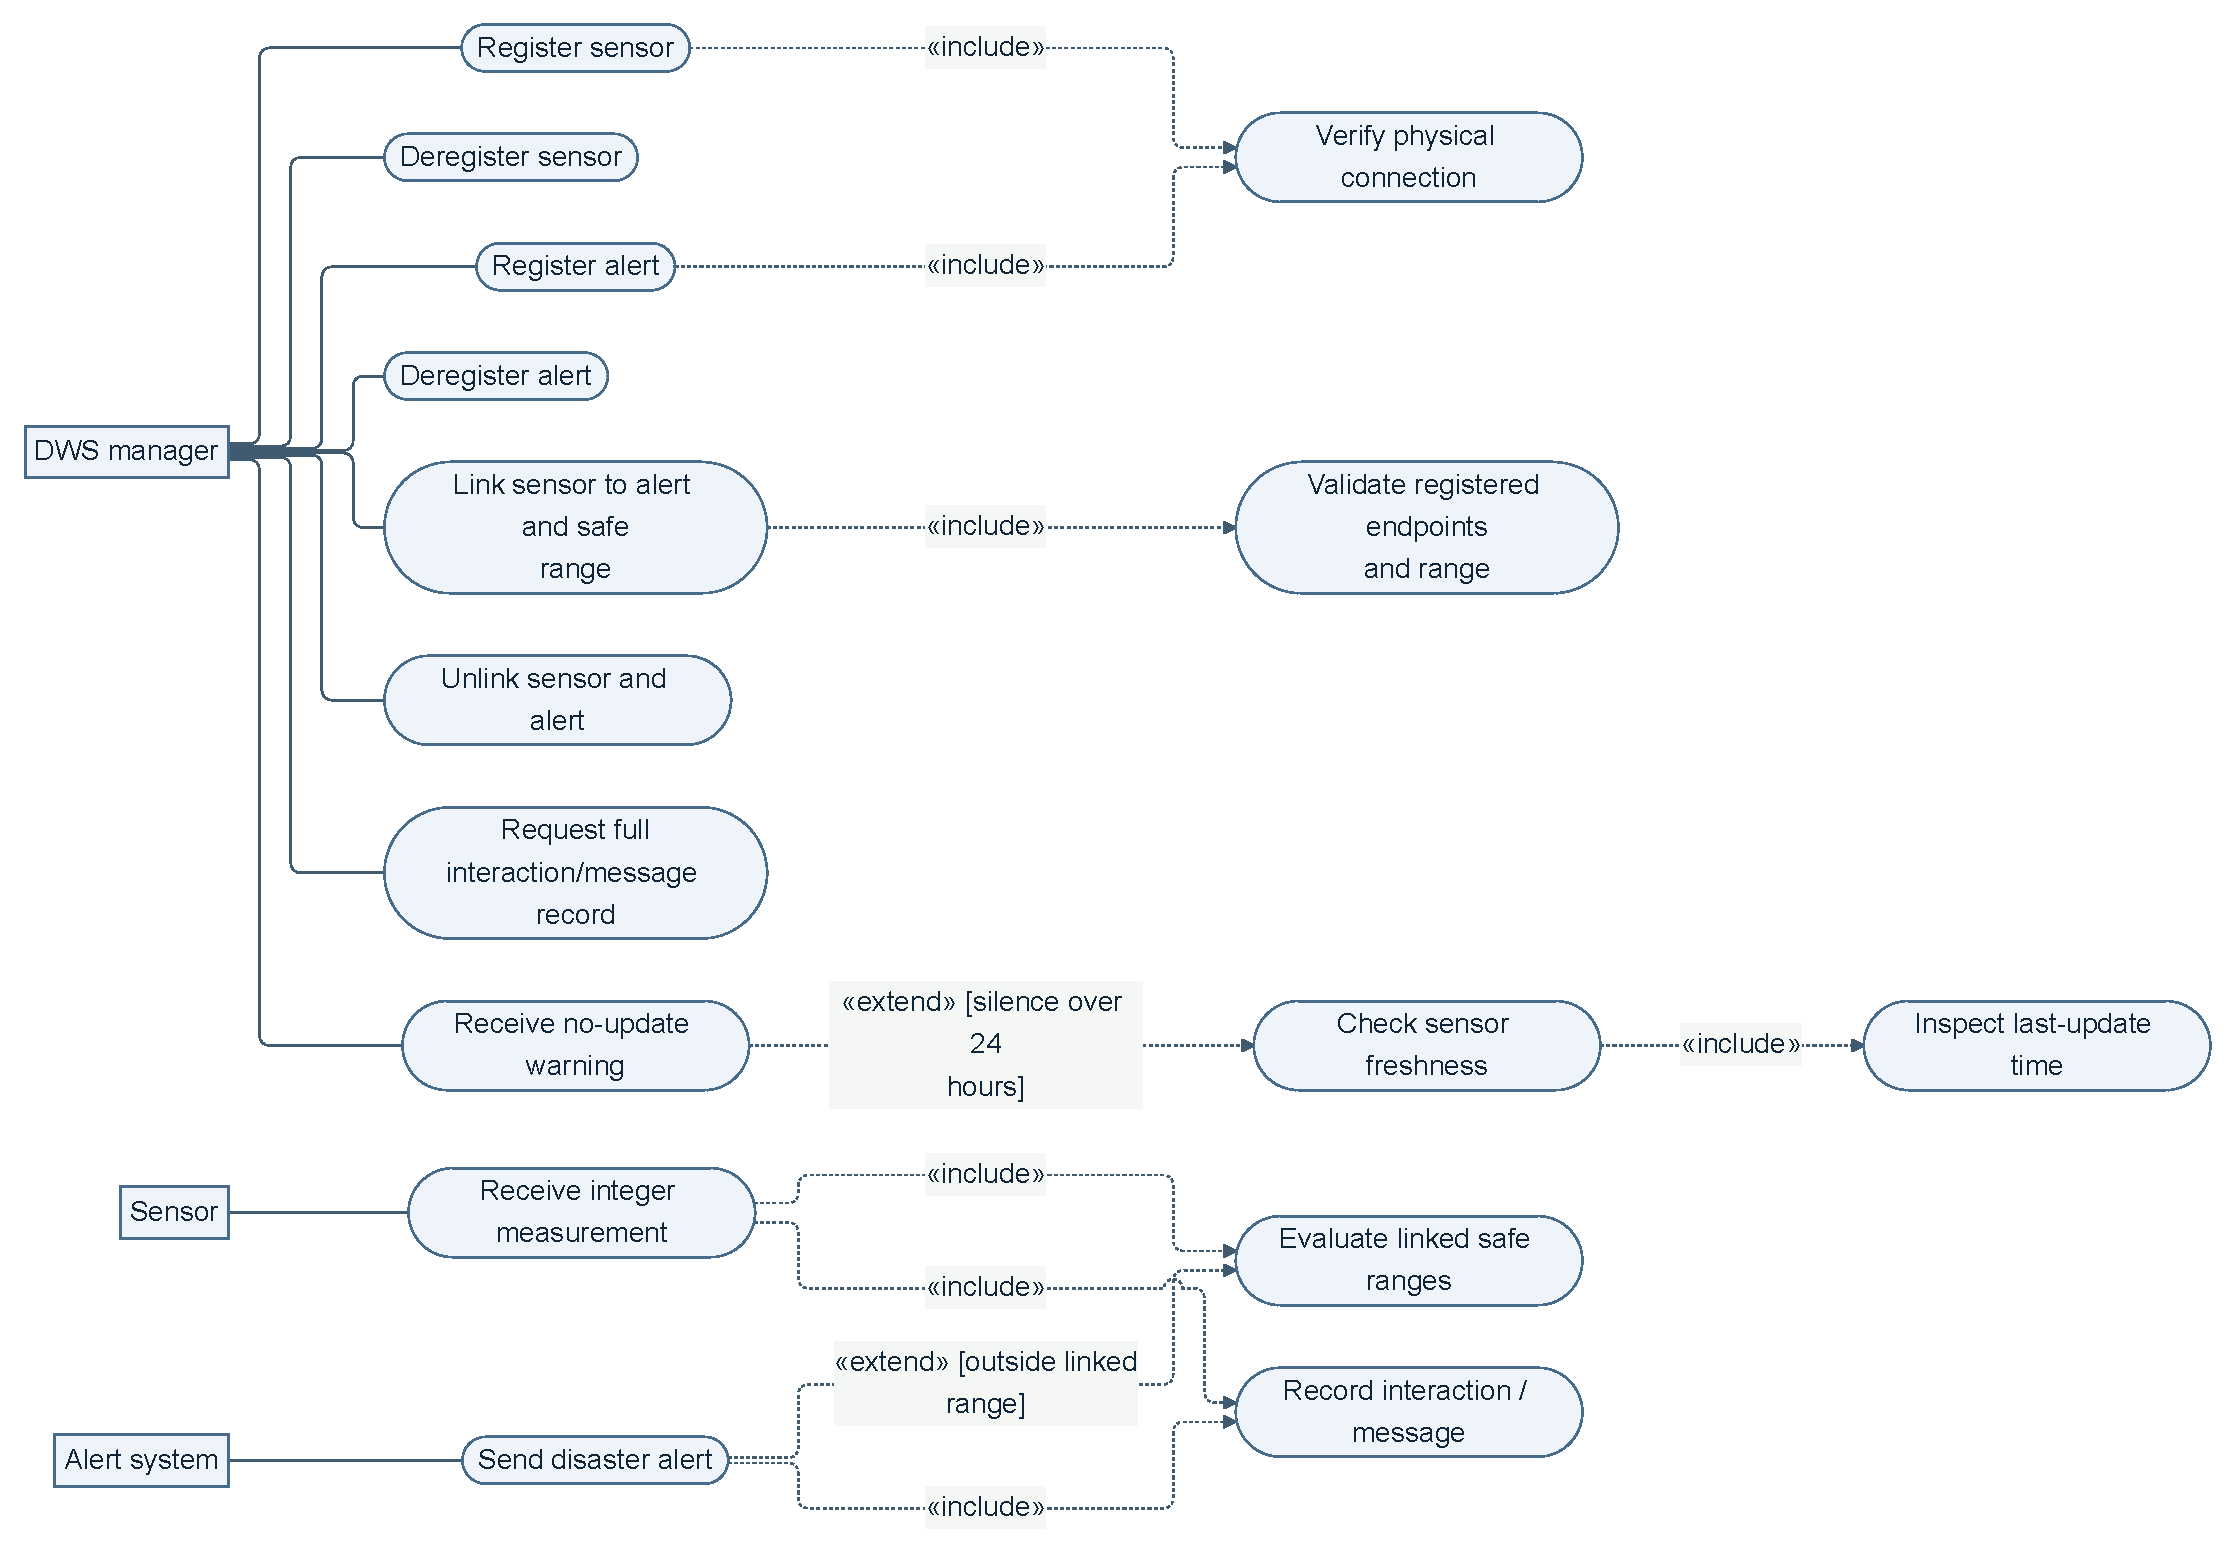
\includegraphics[width=514.00pt]{images/fig-075.pdf}
\captionof{figure}{Q1 --- Stakeholders, requirements and use cases (25 marks)}\end{minipage}\par\smallskip

\begin{studycolumns}
\vspace{0pt}













Registration, deregistration, linking and unlinking also include recording; add their arrows to the shared Record use case in exact UML. The physical-connection check applies only to registration. Safe-range alerting is conditional, making \code{\guillemotleft{}extend\guillemotright{}} reasonable here. The system must not let an unregistered sensor bypass its configured registration policy.

\needspace{4\baselineskip}
\subsection*{Q2 --- Sensor behaviour and process (25 marks)}
\sectionlabel{h-q2--sensor-behaviour-and-process-25-marks}
\textbf{(a) Sensor-object state machine (6). (b) Linking activity/\allowbreak{}swimlanes (7). (c)(i) Choose Waterfall or Agile for changing requirements (3); (ii) manage changes (3). (d) Scrum response to an urgent mid-sprint feature request (6).}


\textbf{(a)} Model the sensor's \textbf{DWS-side lifecycle}, since this software cannot dictate the internal hardware's physical operating states. A registered sensor is monitored even when quiet; silence is not automatic deregistration. A registration timestamp starts monitoring until the first update, a necessary stated assumption because the appendix does not define that initial timer.
\end{studycolumns}


\par\smallskip\noindent\begin{minipage}{\linewidth}\centering
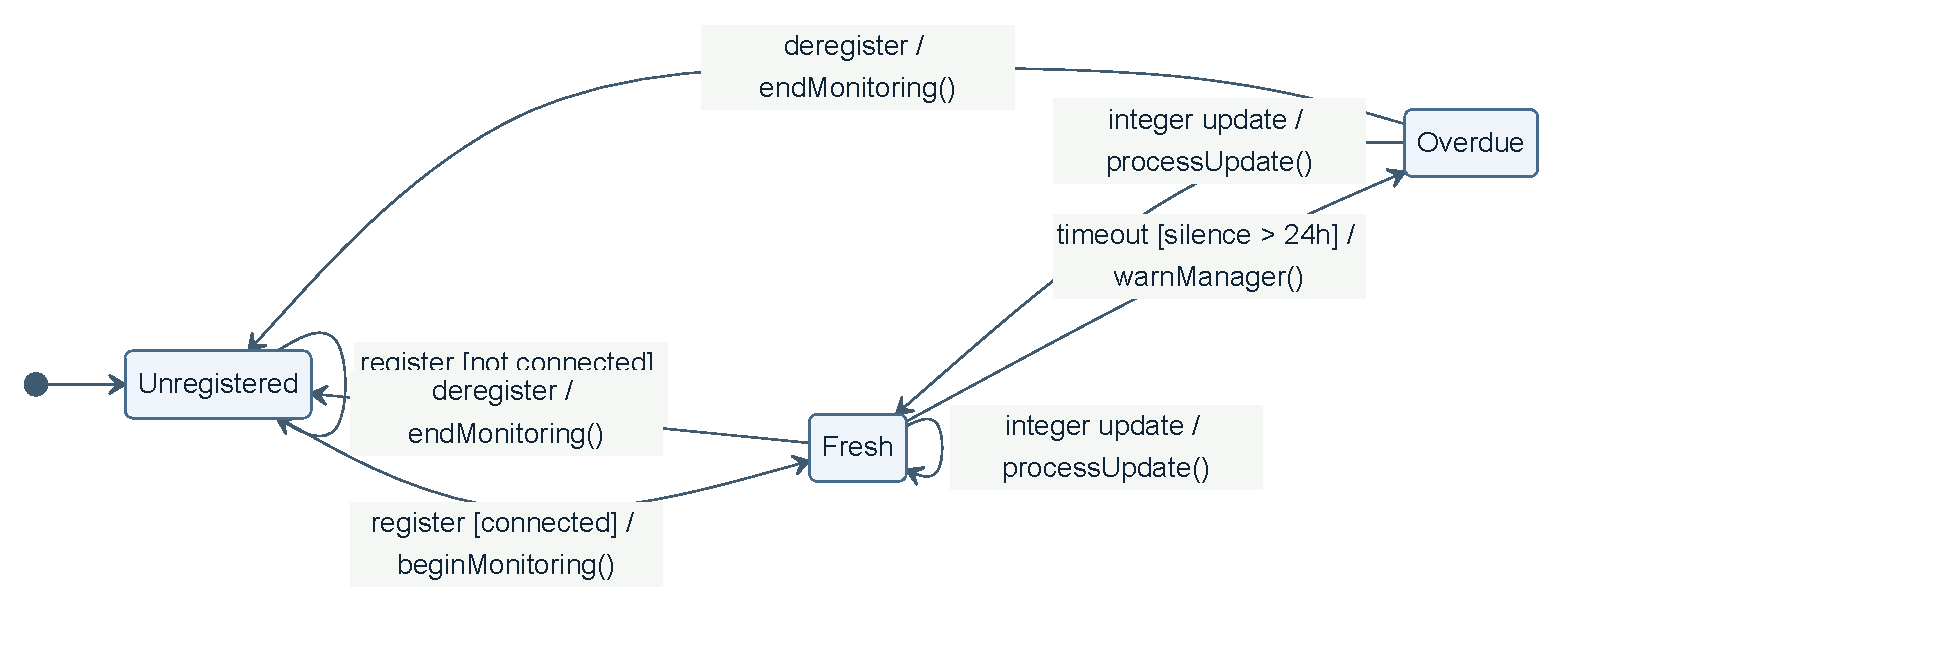
\includegraphics[width=514.00pt]{images/fig-076.pdf}
\captionof{figure}{Q2 --- Sensor behaviour and process (25 marks)}\end{minipage}\par\smallskip





\code{begin\allowbreak{}Monitoring()} records registration and starts freshness timing; \code{process\allowbreak{}Update()} records the valid measurement, evaluates linked ranges and resets freshness; \code{end\allowbreak{}Monitoring()} records deregistration and stops monitoring/\allowbreak{}subscriptions. Exactly 24 hours is not ``over 24 hours''. Repeated warning frequency is unspecified; assume one warning per overdue episode unless the client defines reminders. Invalid-type messages are rejected/\allowbreak{}logged by a defensive integration boundary, not treated as valid measurements.

\textbf{(b)}






\par\smallskip\noindent\begin{minipage}{\linewidth}\centering
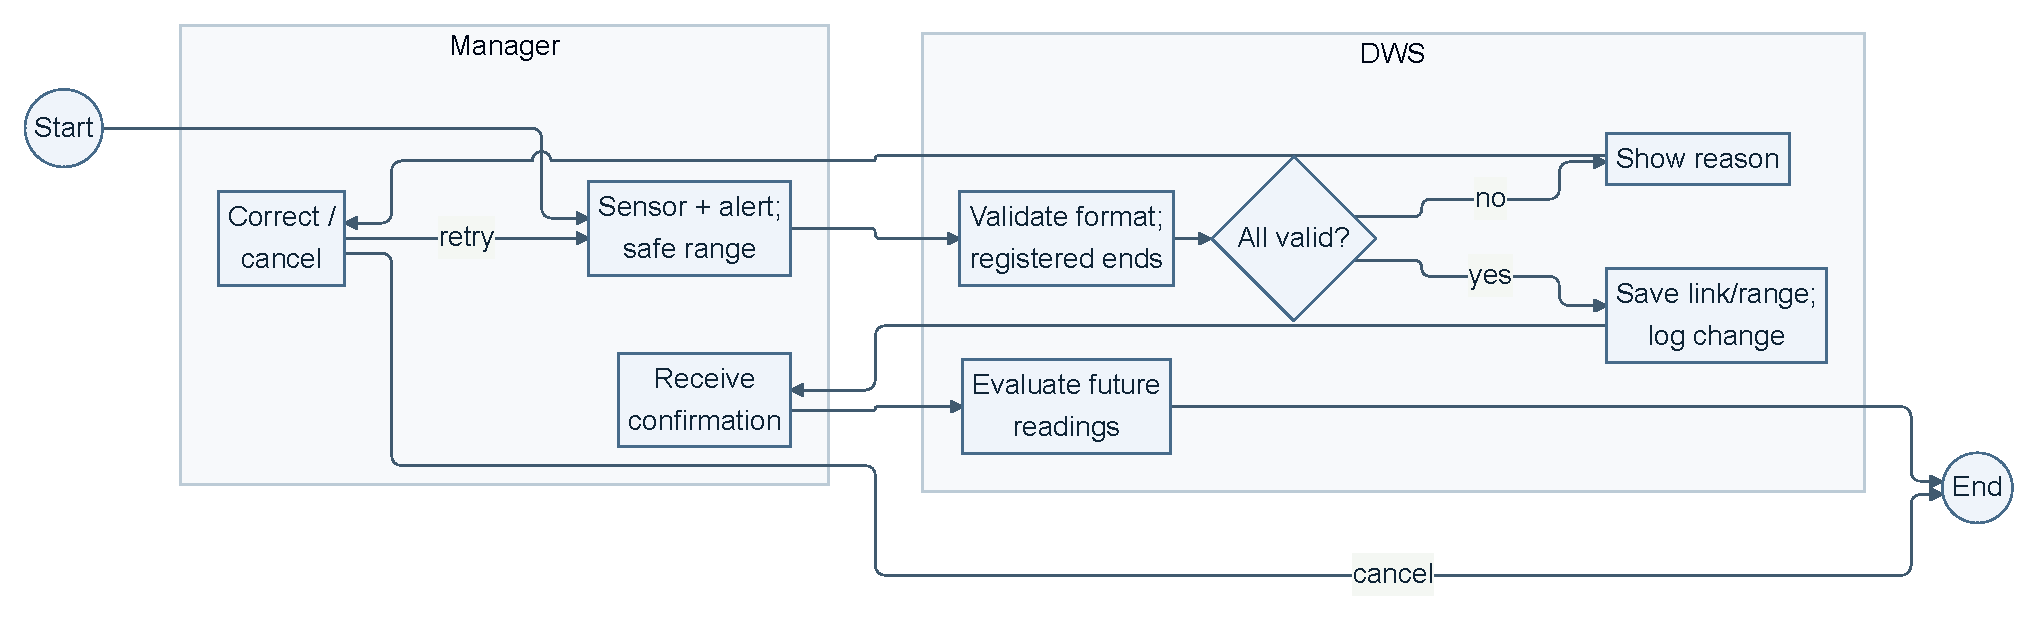
\includegraphics[width=514.00pt]{images/fig-077.pdf}
\captionof{figure}{Q2 --- Sensor behaviour and process (25 marks)}\end{minipage}\par\smallskip

\begin{studycolumns}
\vspace{0pt}









Linking does not require an immediate disaster measurement, nor does it automatically send an alert. Preserve the existing configuration if validation fails.

\textbf{(c)(i)} Recommend Agile/\allowbreak{}incremental delivery because requirements may change and early stakeholder feedback can refine configuration and warning workflows. Retain appropriate safety reviews, documentation and rigorous testing; ``agile'' does not mean no planning.

\textbf{(c)(ii)} Capture changes in a prioritised backlog, clarify acceptance criteria, analyse safety/\allowbreak{}interface impacts and select feasible increments. Protect the current sprint's goal; negotiate later scope and re-estimate affected work, then validate changes with regression and acceptance tests.

\textbf{(d)} Use \hyperref[answer-scrum]{S, p.\ \pageref{answer-scrum}}: PO/developers assess urgency and goal impact; normally backlog the feature for a later sprint. Negotiate transparent scope changes; only the PO cancels an obsolete goal.

\needspace{4\baselineskip}
\subsection*{Q3 --- DWS architecture, Observer and responsibility (25 marks)}
\sectionlabel{h-q3--dws-architecture-observer-and-responsibility-25-marks}
\textbf{(a) Architecture/\allowbreak{}justification (3). (b)(i) Most applicable pattern (3); (ii) detailed classes (10). (c)(i) One reason for/\allowbreak{}against blaming the vendor for a crash on a string measurement (2); (ii) two other responsible parties (4); (iii) three prevention/\allowbreak{}risk-reduction measures (3).}


\textbf{(a)} An event-driven architecture, with layered configuration, monitoring/\allowbreak{}domain and device-integration services, fits asynchronous measurements. A registry manages runtime membership, a monitor evaluates configured links, and gateways deliver alerts while a record store preserves interactions. Isolate malformed or failing devices so one sensor cannot crash monitoring for all others.

\textbf{(b)(i)} \textbf{Observer}: sensor subjects publish measurements to a DWS observer that can subscribe/\allowbreak{}unsubscribe at runtime. This avoids tight coupling to a fixed sensor set and avoids requiring the DWS to synchronously poll for every update. Distinguish domain registration from subscription: the registration service coordinates both, but a list of objects alone is not Observer.

\textbf{(b)(ii)}
\end{studycolumns}


\par\smallskip\noindent\begin{minipage}{\linewidth}\centering
{\scriptsize\textbf{Observer protocol}}\par\smallskip
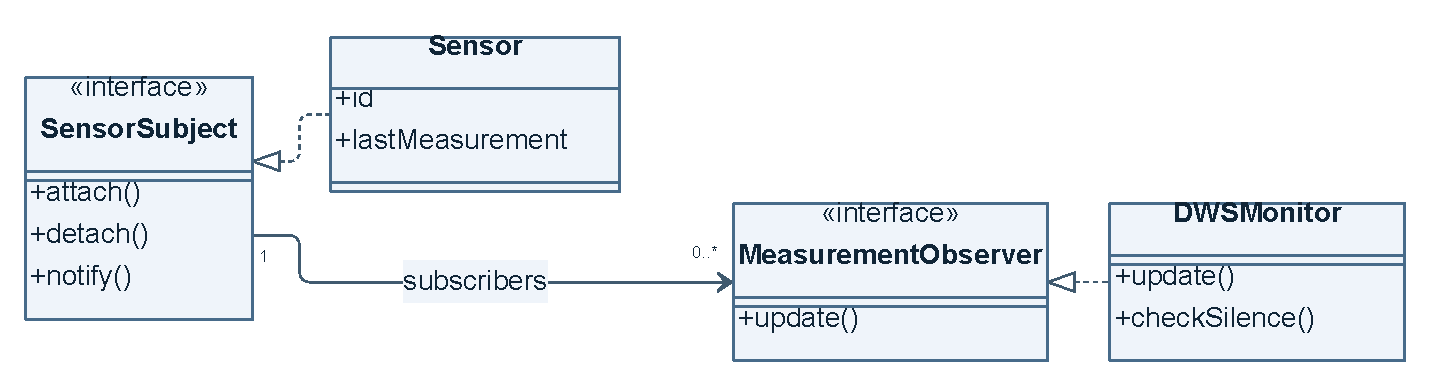
\includegraphics[width=366.00pt]{images/fig-078-protocol.pdf}\par\smallskip
{\scriptsize\textbf{DWS collaborations; DWSMonitor is shared}}\par\smallskip
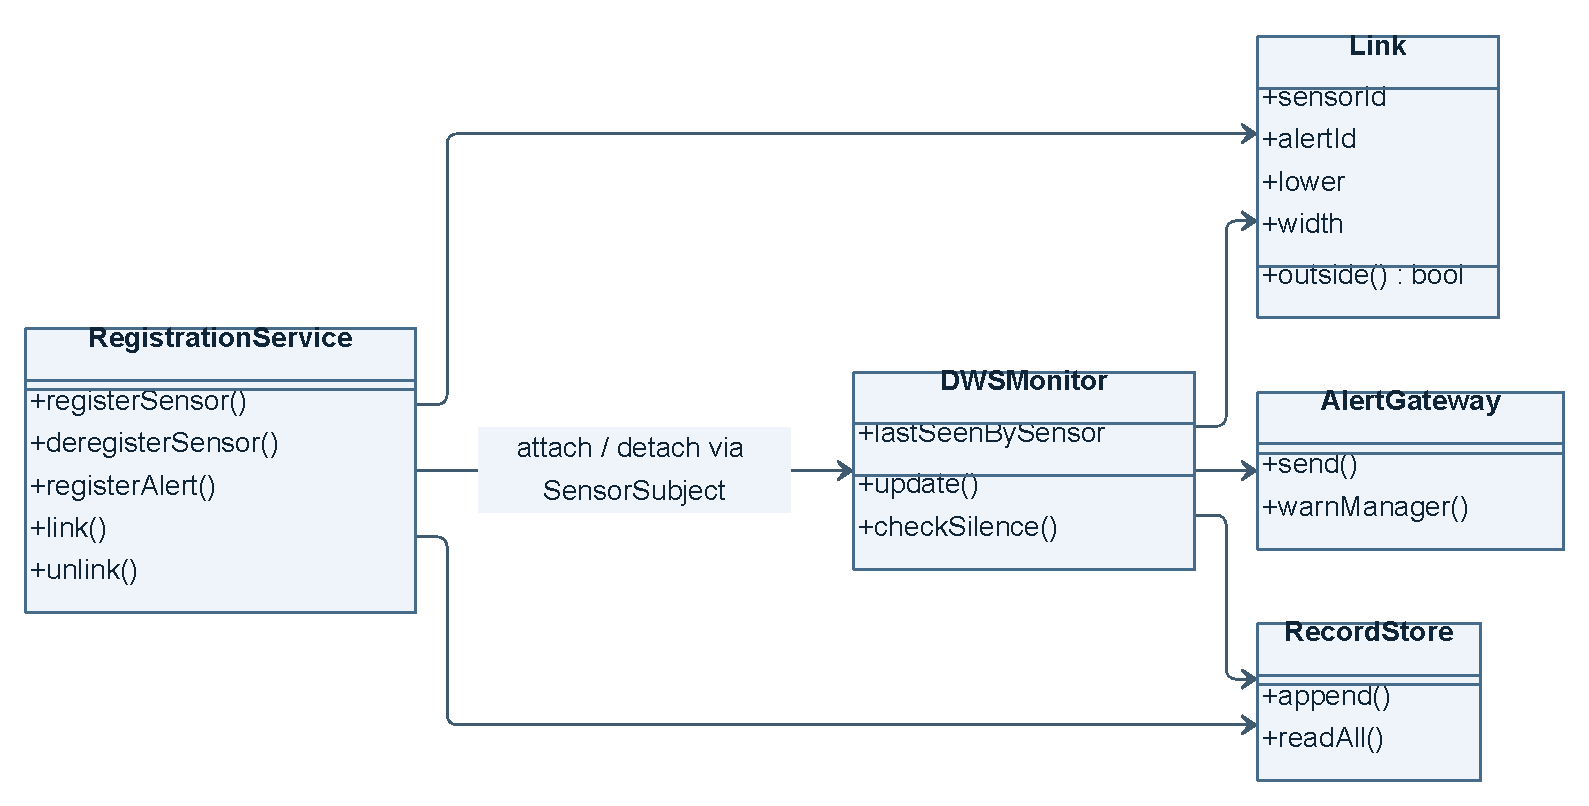
\includegraphics[width=406.80pt]{images/fig-078-services.pdf}\par\smallskip
\captionof{figure}{Q3 --- DWS architecture, Observer and responsibility (25 marks)}\end{minipage}\par\smallskip

\begin{studycolumns}
\vspace{0pt}









For heterogeneous external devices, a sensor adapter can expose SensorSubject while translating the real protocol. \code{update} validates integer messages, records them, updates freshness, evaluates every matching Link, and records any sent alerts. Registration verifies connection before subscribing. Link changes are recorded. Deregistration stops monitoring/\allowbreak{}subscriptions; the policy for dependent links must be agreed rather than leaving dangling references. Use overflow-safe arithmetic for safe-range calculations.

\textbf{(c)(i)} Engineering arguments \textbf{for} responsibility: a foreseeable malformed external input should be rejected/\allowbreak{}isolated rather than causing a system-wide outage, especially in a warning system. \textbf{Against:} the third-party sensor violated the specified integer interface contract; the DWS vendor did not control that sensor's implementation. Both facts can be relevant; neither alone settles all responsibility.

\textbf{(c)(ii)} Sensor manufacturer: emitted a value outside the agreed protocol or failed to validate its output. Client/\allowbreak{}integrator: installed or approved incompatible equipment without verifying conformance and deployment integration. Explain the actual contribution rather than assigning blame solely because a party exists.

\textbf{(c)(iii)} Three measures: (1) validate types/\allowbreak{}ranges and contain exceptions at every device boundary; (2) run defensive, fault-injection and third-party conformance/\allowbreak{}integration tests, including string messages and disconnected devices; (3) document interface contracts, supported-device requirements and acceptance evidence, with monitoring and clear failure reporting. Documentation reduces ambiguity but does not substitute for robust error handling.

\needspace{4\baselineskip}
\subsection*{Q4 --- DWS defensive tests and dependent inputs (25 marks)}
\sectionlabel{h-q4--dws-defensive-tests-and-dependent-inputs-25-marks}
\textbf{Given:} deployed sensor \code{smoke concentration}, alert \code{fire}; signed five-digit decimal \code{N} (e.g. \code{+83220}, \code{-\allowbreak{}00123}); unsigned five-digit non-negative decimal \code{M} (e.g. \code{12345}, \code{00020}). Safe upper bound is \code{N+M}. Individually, integer values outside \code{\ensuremath{-}32768\ldots{}32767} must be rejected.

\textbf{(a) ECs for the four inputs (5). (b) Boundary triplets (4). (c) Defensive test suite (8). (d) Consequences of additionally restricting \code{N+M} to signed 16-bit range (4). (e)(i) Difficulty of one generic deployment-independent suite (2); (ii) solution (2).}


\textbf{(a) Treat formatting and parsed numeric value separately.} Assume exactly one sign and five ASCII digits for N, and exactly five ASCII digits without a sign for M. Leading zeroes are required/\allowbreak{}allowed as in the paper. ASCII names must also identify registered endpoints in this deployment.
\end{studycolumns}


{\fontsize{8.5}{9.8}\selectfont
\begin{longtable}{L{\dimexpr 0.19522\linewidth-4.69pt\relax}L{\dimexpr 0.34556\linewidth-8.29pt\relax}L{\dimexpr 0.45922\linewidth-11.02pt\relax}}
\toprule
\rowcolor{ice}\textbf{Field} & \textbf{Valid EC} & \textbf{Invalid ECs} \\
\midrule\endfirsthead
\toprule\rowcolor{ice}\textbf{Field} & \textbf{Valid EC} & \textbf{Invalid ECs} \\
\midrule\endhead
\multicolumn{3}{r}{\scriptsize Continued on next page}\\\endfoot
\bottomrule\endlastfoot
Sensor name & Exact registered name \code{smoke concentration} & Other ASCII name not registered; name containing non-ASCII characters \\
Alert name & Exact registered name \code{fire} & Other ASCII name not registered; name containing non-ASCII characters \\
N & Format \code{[+-\allowbreak{}][0-\allowbreak{}9]\{5\}} and parsed value \code{\ensuremath{-}32768 \ensuremath{\leq} N \ensuremath{\leq} 32767} & Well-formed value below \ensuremath{-}32768; well-formed value above 32767; malformed representation \\
M & Format \code{[0-\allowbreak{}9]\{5\}} and parsed value \code{0 \ensuremath{\leq} M \ensuremath{\leq} 32767} & Well-formed value above 32767; malformed representation, including a negative/\allowbreak{}sign-bearing input \\
\end{longtable}
}

These partitions are disjoint when numeric invalid classes are restricted to correctly formatted values. \code{+83220} illustrates the required shape but is \textbf{invalid under the additional 16-bit rule}. Negative M cannot satisfy its unsigned format. No assumption that every ASCII name is registered is allowed.

\textbf{(b)} Numeric triplets, written using the required formats:




{\fontsize{8.5}{9.8}\selectfont
\begin{longtable}{L{\dimexpr 0.24105\linewidth-7.71pt\relax}L{\dimexpr 0.26405\linewidth-8.45pt\relax}L{\dimexpr 0.24835\linewidth-7.95pt\relax}L{\dimexpr 0.24655\linewidth-7.89pt\relax}}
\toprule
\rowcolor{ice}\textbf{Boundary} & \textbf{Just below} & \textbf{On boundary} & \textbf{Just above} \\
\midrule\endfirsthead
\toprule\rowcolor{ice}\textbf{Boundary} & \textbf{Just below} & \textbf{On boundary} & \textbf{Just above} \\
\midrule\endhead
\multicolumn{4}{r}{\scriptsize Continued on next page}\\\endfoot
\bottomrule\endlastfoot
N minimum \ensuremath{-}32768 & \code{-\allowbreak{}32769} reject & \code{-\allowbreak{}32768} accept & \code{-\allowbreak{}32767} accept \\
N maximum 32767 & \code{+32766} accept & \code{+32767} accept & \code{+32768} reject \\
M minimum 0 & \code{-\allowbreak{}00001} reject (format) & \code{00000} accept & \code{00001} accept \\
M maximum 32767 & \code{32766} accept & \code{32767} accept & \code{32768} reject \\
\end{longtable}
}

\begin{studycolumns}
\vspace{0pt}

Name membership has no ordered boundary. Extra/\allowbreak{}missing digits and signs are format tests, not numeric boundary neighbours. The just-below-zero M representation is necessarily invalid in format; there is no negative, unsigned, well-formed M string.

\textbf{(c)} In this initial version, the \textbf{sum has no extra 16-bit rejection rule}. For each row keep all other inputs valid. Abbreviations in the table: \code{S =\allowbreak{} smoke concentration}, \code{A =\allowbreak{} fire}; \code{other sensor} and \code{other alert} are stipulated unregistered. A means accepted link/\allowbreak{}configuration, R means clean rejection without changing links or crashing.
\end{studycolumns}


{\fontsize{8.5}{9.8}\selectfont
\begin{longtable}{L{\dimexpr 0.18697\linewidth-7.48pt\relax}L{\dimexpr 0.18697\linewidth-7.48pt\relax}L{\dimexpr 0.18697\linewidth-7.48pt\relax}L{\dimexpr 0.18697\linewidth-7.48pt\relax}L{\dimexpr 0.25211\linewidth-10.08pt\relax}}
\toprule
\rowcolor{ice}\textbf{Sensor} & \textbf{Alert} & \textbf{N} & \textbf{M} & \textbf{Expected /\allowbreak{} purpose} \\
\midrule\endfirsthead
\toprule\rowcolor{ice}\textbf{Sensor} & \textbf{Alert} & \textbf{N} & \textbf{M} & \textbf{Expected /\allowbreak{} purpose} \\
\midrule\endhead
\multicolumn{5}{r}{\scriptsize Continued on next page}\\\endfoot
\bottomrule\endlastfoot
S & A & \code{+00000} & \code{00020} & A --- baseline \\
S & A & \code{-\allowbreak{}32768} & \code{00000} & A --- N lower, M lower \\
S & A & \code{-\allowbreak{}32767} & \code{00001} & A --- valid lower neighbours \\
S & A & \code{+32766} & \code{32766} & A --- valid upper neighbours; sum restriction absent \\
S & A & \code{+32767} & \code{32767} & A --- valid maxima; sum restriction absent \\
S & A & \code{-\allowbreak{}32769} & \code{00020} & R --- N too small \\
S & A & \code{+32768} & \code{00020} & R --- N too large \\
S & A & \code{+00000} & \code{32768} & R --- M too large \\
S & A & \code{+00000} & \code{-\allowbreak{}00001} & R --- M negative /\allowbreak{} forbidden sign \\
other sensor & A & \code{+00000} & \code{00020} & R --- sensor not registered \\
\code{fum\'{e}e} & A & \code{+00000} & \code{00020} & R --- sensor non-ASCII \\
S & other alert & \code{+00000} & \code{00020} & R --- alert not registered \\
S & \code{feu-\allowbreak{}\'{e}} & \code{+00000} & \code{00020} & R --- alert non-ASCII \\
S & A & \code{00000} & \code{00020} & R --- N missing sign \\
S & A & \code{+0000} & \code{00020} & R --- N too few digits \\
S & A & \code{+000000} & \code{00020} & R --- N too many digits \\
S & A & \code{+00a00} & \code{00020} & R --- N non-digit \\
S & A & \code{+00000} & \code{+00020} & R --- M forbidden sign \\
S & A & \code{+00000} & \code{0020} & R --- M too few digits \\
S & A & \code{+00000} & \code{000020} & R --- M too many digits \\
S & A & \code{+00000} & \code{00a20} & R --- M non-digit \\
\end{longtable}
}

\begin{studycolumns}
\vspace{0pt}

Use fresh/\allowbreak{}reset fixtures for each row so an existing link does not alter the oracle. Exactly one \textbf{parameter} is invalid in each rejected row; a malformed parameter can violate more than one format predicate. Supplement with physical-connection/\allowbreak{}registration tests at the appropriate integration boundary.

\textbf{(d)} Now M's valid numeric range depends on N:

\code{0 \ensuremath{\leq} M \ensuremath{\leq} min(32767,\allowbreak{} 32767 \ensuremath{-} N)}, with valid N already in \code{\ensuremath{-}32768\ldots{}32767}.

The sum cannot underflow because M is non-negative, but it can overflow. Partition the \textbf{pair} \code{(N,\allowbreak{}M)} into sum-valid and sum-too-large cases in addition to independent format/\allowbreak{}range classes. For N=\code{+32760}, M=\code{00006}, \code{00007}, \code{00008} exercise below/\allowbreak{}on/\allowbreak{}above the upper sum boundary; the last is now rejected. At N=\code{+32767}, only M=\code{00000} is valid. Reclassify earlier maximum-pair tests rather than reusing their old acceptance oracles. Compute the sum in a wider/\allowbreak{}checked representation before testing its range.

\textbf{(e)(i)} Registered names and even available devices vary by deployment. A name valid in one installation can be invalid in another; a supposedly ``invalid'' hard-coded name may actually be registered elsewhere. Physical connections and existing links also affect results.

\textbf{(e)(ii)} Parameterise the suite with known registered names, verified absent ASCII names and resettable configuration. Prefer a controlled fixture that registers a test sensor and alert (using connected simulators/\allowbreak{}test devices), runs the suite, and restores state. Validate fixture preconditions; do not label deployment differences as software defects.
\end{studycolumns}
